\chapter{Estado del arte}
\label{chap:estadodelarte}

\lsection{Privacidad y anonimato: conceptos}
\label{sec:conceptos}
La privacidad es un concepto bastante complejo, una palabra con tantas acepciones que en algunos casos puede resultar engañosa o, incluso, sin sentido alguno. Los temas donde se trata éste concepto van desde las leyes y derechos hasta la tecnología, pasando por campos tan ambiguos como la filosofía.

Por otro lado, el contexto en el que suele ser utilizada va desde los ajustes de un navegador hasta uno de los debates más importantes sobre el desarrollo de la sociedad.

En resumen, los usos del concepto de privacidad abarcan un número incalculable de temas y es por ello por lo que dicho término es difícil de definir. 
Sin embargo, en este proyecto nos atañe el uso relacionado con la red, y aquí se puede definir como el control de la información que posee un determinado usuario que se conecta a Internet, interactuando con diversos servicios en línea con los que intercambia datos durante la navegación. 

Cabe mencionar que muchos de los usuarios que navegan día a día no son realmente conscientes de los datos personales que circulan por la red.

\begin{figure}[h]
	\centerline{
		\mbox{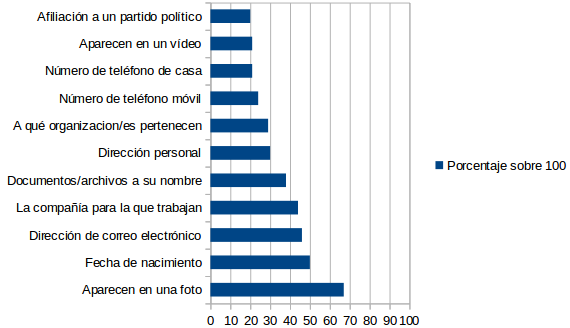
\includegraphics[width=5.00in]{images/chart_privacy.png}}
	}
	\caption{Resultados del estudio en Pew Research Center's and American Life Project hecho en Julio de 2014}
	\label{fig:norm_Daugman}
\end{figure}

La privacidad no debe confundirse con el \textbf{anonimato en la red}. Éste último término refiere a aquellas acciones destinadas a garantizar que el acceso a la red se efectúa de forma que no se conoce quien realiza la conexión.

Por último conviene hablar de otra expresión que aparecerá también muy frecuentemente en este proyecto, y es el de \textbf{ofuscación}.

En su sentido más abstracto, la ofuscación es la producción de ruido modelado en una señal existente con el objetivo de hacer una recopilación de datos más ambigua, confusa, difícil de \textit{explotar} y, por ende, menos valiosa.

\subsection{Procedimientos para incrementar el anonimato}

Este subcapítulo tiene como objetivo explicar los distintos tipos de procedimientos para lograr un mayor grado de anonimato en la red. 

Antes de nada conviene diferenciar dos conceptos comúnmente confundidos como son el de pseudoanonimato (\textit{pseudonymity} en inglés) y anonimato.

El primero de ellos refiere al hecho de usar un pseudónimo con el fin de camuflar una identidad real. Su significado literal según su etimología es  "llamado engañosamente".
Por otra parte, el segundo, cuyo origen etimológico significa "sin nombre", refiere cuando no hay información identificable a nada ni nadie.

Por ende, la principal diferencia entre ambos términos radica en que mientras en el anonimato la identidad es totalmente desconocida, en el pseudoanonimato se aprovecha el hecho de utilizar un pseudónimo para esconder una identidad real. 
En éste proyecto se ha trabajado con métodos tanto para lograr un anonimato como para lograr un pseudoanonimato.

Una vez aclarados sendos términos, procedemos a listar las diferentes vías para lograr el anonimato:

\begin{itemize}
	\item Anonimato de emisor: Este tipo consiste en un origen que efectúa un mensaje a un determinado receptor, y el emisor no puede ser reconocido por ningún observador.
	\item Anonimato de receptor: En este caso, al contrario del anterior, es el receptor el que no puede ser identificado por el observador.
	\item Anonimato de comunicación: Este capítulo trata con detalle la fase de diseño, teniendo en cuenta la estructura de la aplicación y el flujo de navegación de la misma 

\end{itemize}

\lsection{Hechos relevantes con respecto a la seguridad en la red} \label{sec:historia}

Conviene empezar el capítulo recalcando que Internet no fue concebido como un protocolo de comunicación seguro. 
Es por esto que a lo largo de su historia han ocurrido varios sucesos que han puesto en riesgo (por diversos motivos) la privacidad del usuario en la red.

Podemos marcar como primera incursión histórica con respecto a la seguridad un libro publicado por Jon Von Neumann en el año 1949 llamado \textit{The Theory of Self Reproducing Automata}. Dicha publicación sirvió como  base para el desarrollo de los primeros \textbf{virus informáticos}.

El primer virus que causó un gran impacto social fue el lamado \textbf{virus Creeper}, el cual era un programa experimental autoreplicante creado por \textbf{Bob Thomas} diseñado con fines experimentales y que no causaba un daño real entre las máquinas en las que se iba moviendo. 
Realmente fue desplazándose de ordenador en ordenador alrededor de toda la red ARPANET (la precursora de lo que es a día de hoy internet).

Con el objetivo de acabar con dicho virus apareció \textbf{Reaper}, lo que hoy día llamaríamos antivirus pero que en realidad no era más que otro programa autoreplicante cuyo propósito era la eliminación de Creeper en cada uno de los sistemas donde se encontraba instalado.

En 1973 Robert Metcalfe, un trabajador de ARPANET y el cuál fundó 3Com (uno de los fabricantes de redes informáticas más importantes), advertía que una incursión a la red interna desde el exterior era algo extremadamente sencillo y, de hecho, son atribuidas durante la década de los 70 varias intrusiones a la red por parte de estudiantes de secundaria. 
Durante esta etapa no se produjeron descubrimientos destacables con respecto a la seguridad informática. De hecho, en el año 1978 un grupo de científicos propusieron un proyecto de cifrado de paquetes TCP/IP pero encontraron muchas trabas, algunas de ellas incluso por la Agencia de Seguridad Nacional. Por ello, dicho proyecto (que bien podría haber marcado otro camino en la historia de la seguridad en la informática) fue abandonado.

En 1981 apareció el segundo virus reconocido a nivel mundial, el llamado \textbf{Elk Cloner}. Atacaba computadoras Apple II, aunque su único propósito era el de reproducirse en otros dispositivos y no efectuaba ningún daño propiamente dicho. Uno de los datos más impactantes es que fue diseñado por un joven de 15 años. Su propagación era mediante el disquete. 
Este virus sentó la base para los siguientes que fueron apareciendo, los cuales contendrían todo tipo de código destructivo (robo de datos, manipulación de los mismos, destrucción de software y hardware...) y se propagarían por más medios, como el correo electrónico e Internet.
Debido a la aparición de los numerosos softwares maliciosos en esta época fueron apareciendo empresas que proporcionaban herramientas para proteger los equipos, los \textbf{antivirus}.

En el año 1983, se hizo mandatorio que los usuarios de la red ARPANET utilizasen el protocolo TCP/IP. Éste hecho estableció un estándar en la comunicación entre redes y favoreció la aparición de la World Wide Web.
Éste fue además el año en el que se utilizó por primera vez el término \textit{virus informático} en una tesis académica, dirigida por Fred Cohen.

En 1986 se aprueba una ley llamada La \textit{Ley De Fraude Y Abuso Cibernético } la cual aparece como contramedida al virus más dañino hasta la fecha como fue Brain, el primer virus compatible con máquinas IBM. La ley defendía a los usuarios del robo de datos, del acceso a la red no autorizado y demás delitos relacionados con la tecnología.

1987 fue un año de grandes avances en el campo de la seguridad informática en todo el mundo.
En primer lugar, se produjo la primera eliminación total de un virus dañino a gran escala por parte de Bernd Fix. 
Por otra parte Andreas Lűning y Kai Figge lanzan al mercado el primer antivirus diseñado para la plataforma Atari.
Además, aparece la primera empresa estadounidense de antivirus, creada por John McAfee. 
Por último, añadir que aparecen los primeros antivirus basados en heurísticas, como son Anti4us y Flushpot.

Los tres años siguientes siguieron apareciendo compañías que velaban por la seguridadm como Symantec, la cual lanzó el conociod antivirus Norton en el año 1991.
Sin embargo, ésto no hizo que el número de robos de información cesara. Al contrario, pues con la aparición del primer navegador web surgieron nuevas formas de ataque y \textit{phising}. Asimismo surgieron los primeros ataques de denegación de servicio.

En el año 1996, con la aparición del complemento de navegador Flash(que permite la reproducción de vídeo y música) surgen por ende nuevas formas de ataques, debido a las numerosas vulnerabilidades del plugin. El correo electrónico, que cada vez se encuentra más vigente, también permite recibir correspondencia con un objetivo de robar información personal. En éste año también aparece el primer virus creado para el sistema Linux, llamado Staog.

El año 2000 el número de gusanos informáticos que se encientran en equipos domésticos es desproporcionado. Asimismo, en ésta década los ciberdelincuentes aprenden a anonimizarse más sofisticadamente y hacen más difícil su identificación.
Para el año 2005 el número de malware únicos asciende a más de 300.000, y ha ascendido más de un 1000\% en diez años. Para el año 2008 dicha cifra asciende 5 millones de malware únicos.

En los últimos años la variedad de ataques de robo de información ha cambiado mucho. Con la aparición de los smartphones, surgen nuevas amenazas para nuestra privacidad como \textit{payloads} que corren como un proceso en segundo plano y permiten tracear nuestra ubicación, espiarnos a través de la cámara del dispositivo y un largo etcétera. Ésto ha ocasionado que surjan también aplicaciones antivirus en nuestros teléfonos móviles, que actúan de forma \textit{pasiva} vigilando que ningún proceso monitorice de forma maliciosa nuestro dispositivo.

Sin embargo, con el incremento del número de amenazas a nuestra privacidad también ha sido necesario que aparezcan herramientas que actúen de forma \textit{activa} y nos permitan utilizar los servicios de Internet de una forma más segura.

	
\lsection{Herramientas para la protección de identidad}
\label{sec:a_favor}

Hoy en día existen numerosas aplicaciones que permiten aumentar nuestro grado de anonimato a la hora de realizar tareas en Internet, usualmente a costa de una más óptima velocidad de conexión,por ejemplo, el servicio \textbf{Tor}, o a cambio de una suscripción temporal, como los \textbf{servicios VPN de pago}.

\subsection{Servidor proxy}

Un servidor proxy es básicamente un mediador entre un usuario que realiza una petición y otro servidor.
Su funcionamiento es relativamente simple: Cuando un cliente de la red desea acceder a un recurso, es el servidor proxy el que realiza la comunicación y el que lleva el resultado de la petición al usuario final. 

Los usos de dicha aplicación en ejecución van desde aumentar el rendimiento de algunas operaciones sirviendo como memoria caché, hasta proteger la identidad del usuario que lo utiliza.
Dicha finalidad depende del tipo de proxy que se esté utilizando.
Hay varios tipos, los cuales se resumen a continuación.

\subsubsection{Proxy Web}

Un \textbf{servicio proxy ó proxy web} es un proxy para una aplicación concreta, y permite el uso de los protocolos FTP y HTTP/S.

Éste tipo de proxy es muy comúnmente utilizado para proteger la privacidad y se puede utilizar junto con Tor (el cual veremos más adelante) para mejorar el grado de anonimato en la red.

El esquema de funcionamiento es el siguiente:

\begin{figure}[h]
	\centerline{
		\mbox{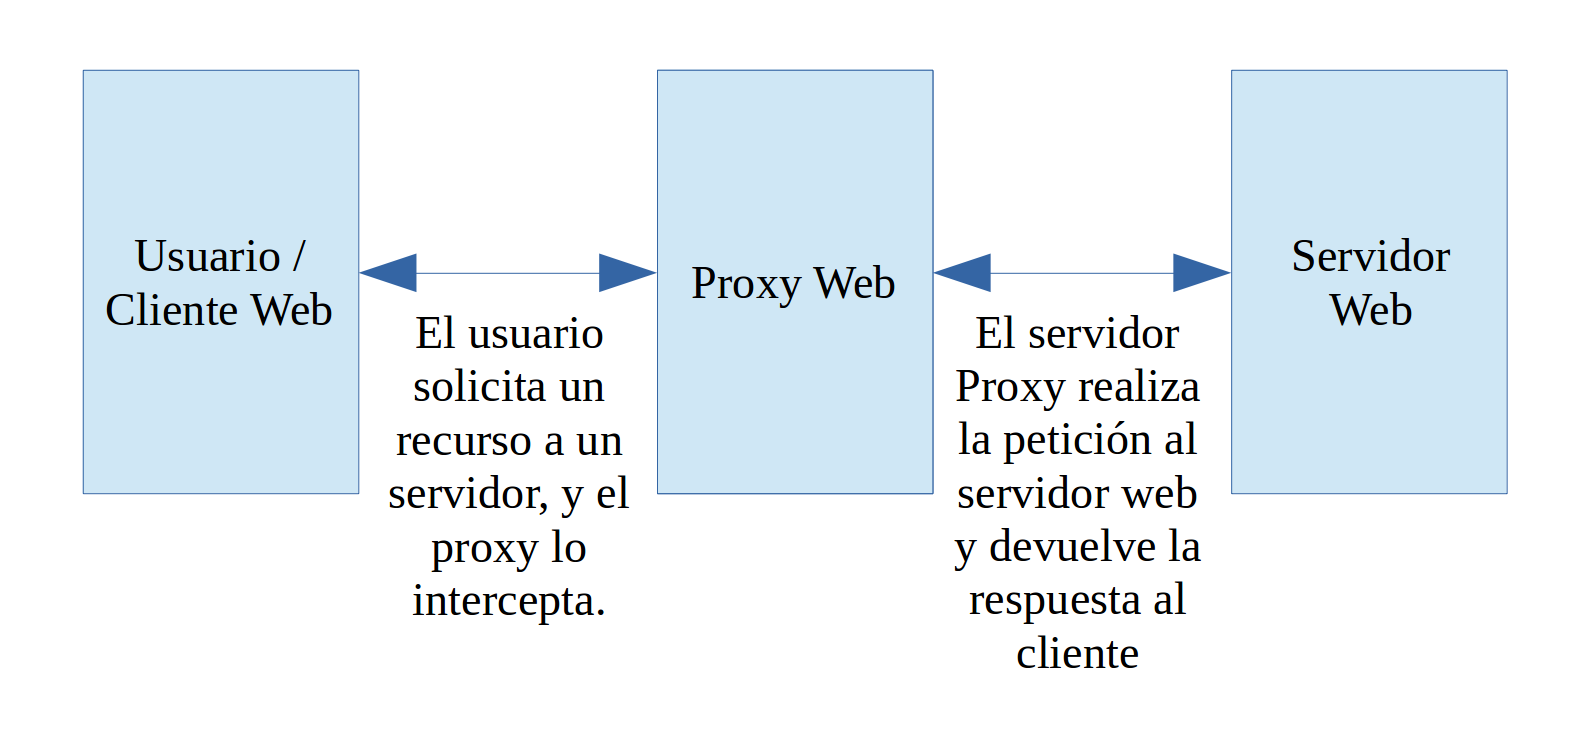
\includegraphics[width=3.00in]{images/proxy_web.png}}
	}
	\caption{Funcionamiento de un Web proxy o Proxy service}
	\label{fig:norm_Daugman}
\end{figure}

\subsubsection{Proxy Cache}

Su propósito es el de guardar el contenido solicitado por el usuario para así mejorar la velocidad de respuesta en futuras solicitudes de recursos. 
Conviene destacar a su vez que un proxy web puede actuar también almacenando las páginas web solicitadas, actuando de cierta manera como un proxy caché. Funciona de la siguiente manera:

\begin{figure}[h]
	\centerline{
		\mbox{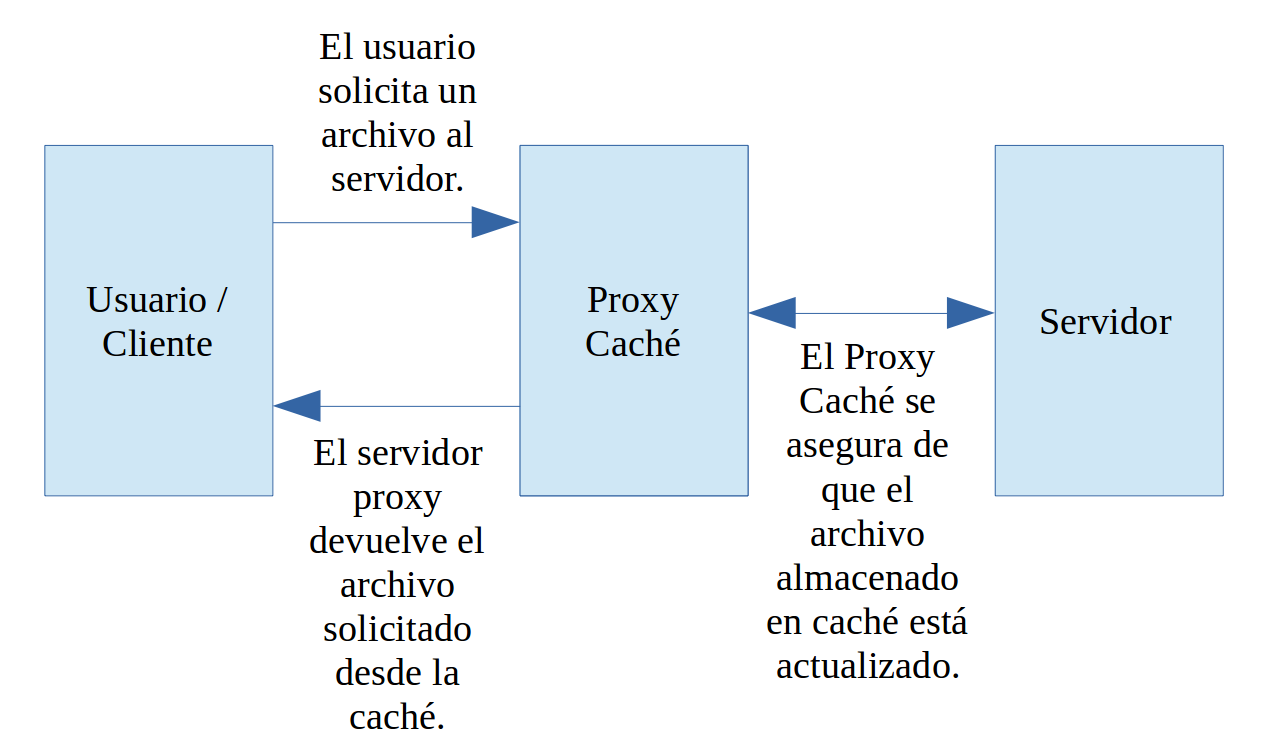
\includegraphics[width=3.00in]{images/proxy_cache.png}}
	}
	\caption{Funcionamiento de un Proxy Caché}
	\label{fig:norm_Daugman}
\end{figure}

\subsubsection{Transparent Proxy}

También es conocido como proxy forzado, y tiene la peculiaridad de no modificar la petición realizada por el cliente ó respuesta más allá de la autenticación del propio proxy.
Se le llama transparente puesto que el usuario final no necesita realizar ningún tipo de configuración adicional en el navegador.
Su uso es principalmente el de filtrar ciertas conexiones (se combina con un \textit{cortafuegos}) y para proporcionar seguridad.

\begin{figure}[h]
	\centerline{
		\mbox{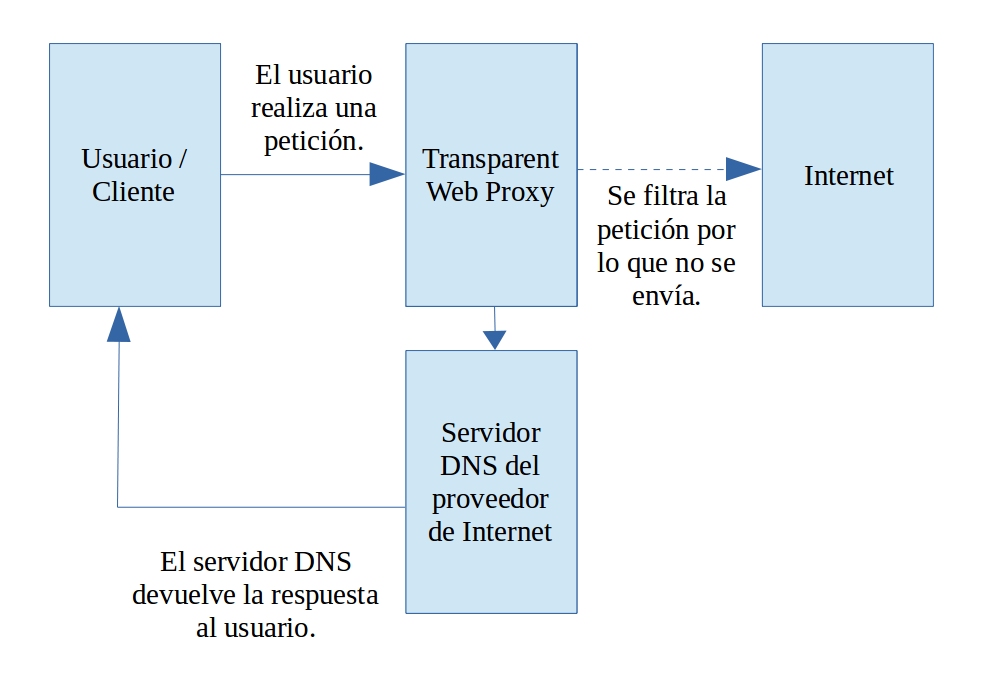
\includegraphics[width=3.00in]{images/proxy_transparent.png}}
	}
	\caption{Funcionamiento de un Proxy transparente}
	\label{fig:norm_Daugman}
\end{figure}

\subsubsection{Reverse Proxy}

Este proxy tiene la peculiaridad de estar alojado en uno o más servidores web.
Es decir, mientras que un proxy normal es el intermediario entre sus clientes para realizar peticiones a cualquier servidor, un proxy inverso es el intermediario entre sus servidores asociados para ser contactados por cualquier cliente.

\subsubsection{NAT proxy ó enmascaramiento}

El uso de este proxy es también llamado \textbf{enmascaramiento de IP}. En este caso, las direcciones de destino de los paquetes IP son reemplazadas por otras. 
En este caso la actuación de mediador es entre los equipos de la red interna y la red exterior.

Los aquí citados son los principales tipos de proxies. No obstante, existen algunos más, como el \textbf{proxy abierto} y el \textbf{Cross-Domain }proxy.

Una vez dejados claros los conceptos básicos sobre proxies, mencionaremos algunas herramientas útiles que hacen uso de éstos para navegar de una forma más anónima y segura por la red.

\subsubsection{Proxychains}

Proxychains es un programa disponible únicamente para GNU/Linux y Unix que nos permite crear cadenas de proxies, escondiendo así nuestra dirección IP pública en \textbf{todo tipo de conexiones} (HTTP, FTP, SSH, etcétera). 
Esto se traduce en que podemos navegar por Internet o realizar cualquier operación en la red de redes sin descubrir nuestra identidad real.

Mientras que en las figuras anteriores mostramos una conexión a la red con la utilización de un sólo proxy, en el caso de \textit{proxychains} (como su propio nombre indica) utilizaremos cadenas de servidores proxy para anonimizar el tráfico que generemos(no necesariamente debe ser tráfico web).

\begin{figure}[h]
	\centerline{
		\mbox{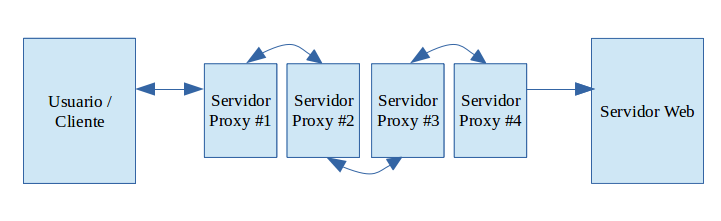
\includegraphics[width=3.00in]{images/proxy_chain.png}}
	}
	\caption{Ejemplo de una cadena de proxies}
	\label{fig:norm_Daugman}
\end{figure}

Para hacer funcionar proxychains en un equipo es necesario modificar su fichero de configuración (\textit{proxychains.conf}). En él existen varias opciones en cuanto a la formación de ccadenas de proxies:

\begin{itemize}
	\item \textit{Dynamic chains}: Supongamos que tenemos 4 servidores proxies añadidos en nuestro archivo de configuración, en este orden: A, B, C y D.
	En el caso de que, por ejemplo, el servidor B esté caído y el resto funcionen perfectamente, la conexión se realizará de la siguiente manera:
	
	\begin{figure}[h]
		\centerline{
			\mbox{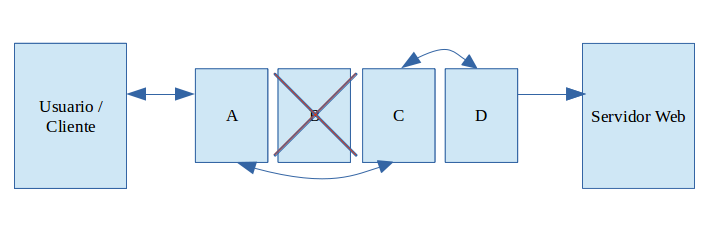
\includegraphics[width=3.00in]{images/proxy_dynamic.png}}
		}
		\caption{Cadena dinámica}
		\label{fig:norm_Daugman}
	\end{figure}
		
	Es decir, aunque uno (o varios) de los servidores proxy que componen la cadena no funcione, siempre se intentará realizar la conexión omitiéndolo.
	
	\item \textit{Strict chains}: Si tomamos el ejemplo anterior, en el caso de una cadena estricta ocurre lo siguiente:
	
	\begin{figure}[h]
		\centerline{
			\mbox{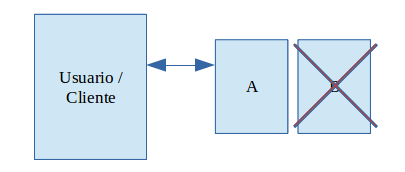
\includegraphics[width=1.80in]{images/proxy_strict.png}}
		}
		\caption{Cadena estricta}
		\label{fig:norm_Daugman}
	\end{figure}
			
	En el caso de que uno de los servidores proxy falle, la conexión no será satisfactoria. Por ello, las cadenas estrictas tienen la peculiaridad de que siguen el orden de los servidores rigurosamente.
	
	\item \textit{Random chains}: Éste tipo de cadenas es totalmente distinta de las anteriores. Básicamente escoge uno de los servidores proxy que aparecen en el archivo de configuración de forma aleatoria.
\end{itemize}

Ahora bien, ¿cómo podemos añadir servidores proxy a nuestra cadena?
El formato para añadirlos es el siguiente:


{\fontfamily{bch}\selectfont 
	socks5  192.168.67.78   1080    user   password
}

El primer elemento es el tipo de proxy. Las posibilidades son HTTP, socks4 y socks5. Como nuestro objetivo es el de anonimizarnos y proteger nuestra identidad \textbf{siempre que sea posible se intentará utilizar socks5}.
El segundo y tercer elemento es la dirección IP y el puerto del proxy, respectivamente. 
Por último, el cuarto y quinto campo son opcionales y depende de si el proxy que utilizaremos cuenta con usuario y contraseña. Normalmente cuentan con contraseña los proxies que adquirimos por medio de plataformas de pago.

Hay una gran cantidad de páginas que ofrecen servidores proxies, tanto gratuitos como de pago. La diferencia radica en la carga de dichos servidores. Muchos de los servidores proxy gratuitos publicados en la red se encuentran saturados y limitan mucho la velocidad de conexión.

No obstante, es posible encontrar servidores proxy gratuitos que funcionan relativamente bien. Una buena página en la que encontrarlos es https://socks-proxy.net/. 
Ésta página permite visualizar servidores proxy gratuitos con disponibilidad actualizada cada 20 minutos. Además, permite filtrarlos según tipo y sobre todo, país de origen.

Con el objetivo de mantenernos anónimos en la red, conviene utilizar proxies ubicados en países que tengan buenas políticas de privacidad. Ejemplo de ello son países como \textbf{Rusia, China o Países Bajos}.

\subsection{VPN}

Una VPN (o red virtual privada) no es más que el uso de una red privada segura sobre una red pública más grande. 
La notoriedad que ha cosechado éstos últimos años reside en que nos permite gozar de un alto grado de anonimato al darnos acceso al envío y recibo de datos de la red pública, teniendo todas las políticas de privacidad de una red privada.

La forma de conseguir esto es, normalmente, estableciendo una conexión extremo a extremo mediante el uso de cifrado y/o conexiones dedicadas.

Pese a que el término se ha visto utilizado enormemente estos últimos años, lo cierto es que las redes privadas virtuales existen desde hace bastante tiempo.
De hecho, la primera forma de VPN surgió con SwIPe (\textit{Software IP Encryption Protocol}), un trabajo experimental surgido en el año 1993 por John Ioannidis y su equipo en la Universidad de Columbia y AT\&T Labs. Éste proyecto pretendía garantizar confidencialidad, integridad y autenticación del tráfico de red.

Tras este experimento, en el año siguiente Xu Wei continuó investigando acerca de la seguridad del protocolo IP hasta formar la familia de protocolos IPSec, la cual autentica y cifra cada paquete compartido a través de una red pública. Después de un tiempo y tras la mejora en las velocidades de transmisión de paquetes, y de la función \textit{plug-and-play}, fue posible la salida al mercado de \textbf{las primeras VPNs}.

A la vez que apareció IPSec, se  realizó un trabajo en la Biblioteca de Investigación NAVAL con ayuda de DARPA (Defense Advanced Research Projects Agency) con el que surgió el \textbf{Protocolo de Seguridad de Encapsulación}. 
Con ello surgió un gran avance para la seguridad en internet y la tecnología VPN. 
La Carga de Seguridad Encapsulada, \textbf{ESP, ofrece la autenticidad, integridad y protección de la confidencialidad de los paquetes de datos}. 
Permite configuraciones de autenticación, encriptación, o ambos. 
Este protocolo es similar al de los Encabezados de Autenticación y proporciona una segunda capa de seguridad para las conexiones a Internet. 

1995 fue el año en el cuál se creó el grupo de trabajo de IPsec dentro de la IETF, o Internet Engineering Task Force, el cual es una comunidad de ingenieros de Internet, proveedores, desarrolladores y otras personas interesadas en la evolución de internet y su buen funcionamiento. 

El objetivo de este grupo era el de crear un conjunto estandarizado de protocolos disponibles libremente y examinados abordando los componentes, extensiones y la implementación de IPsec.

IPsec está formado por tres subprotocolos:

\begin{itemize}
	\item \textit{Autentication Header (AH)}: Este protocolo es el encargado de proporcionar integridad de datos en el caso de no haber conexión y autenticación de paquetes IP, además de protección contra ciertos tipos de ataques. 
	La \textbf{autenticación} es importante porque asegura que los paquetes de datos que envías y recibes son los que deseas, no el malware u otros ataques potencialmente dañinos. Hay varias versiones con diferentes grados de protección a diferentes niveles. En todos los casos, la Carga de Paquetes IP, tus datos personales están protegidos.
		
 	\item \textit{Encapsulating Security Payload (ESP)}: Se ocupa de proporcionar la confidencialidad de esos paquetes, al igual que integridad de origen de los datos, la seguridad a los ataques y también seguridad para el tráfico de flujo. Cuando se utiliza en \textbf{Modo Túnel}, proporciona seguridad para todo el Paquete IP.
 	
	\item \textit{Security Associations (SA)}: Son algoritmos y datos que permiten que AH y ESP funcionen correctamente. 
	Básicamente, los datos se cifran en paquetes en la fuente y luego se transfieren a través de internet de forma \textbf{anónima} para ser recibidos, autenticados y descifrados en el destino. Las asociaciones se crean sobre la base de la Internet Security Association And Key Management Program (ISKAMP) utilizando una serie de números.
\end{itemize}

Además de esto, existen dos modos de funcionamiento:

\begin{itemize}
	\item \textit{Transport Mode}: En Modo Transporte únicamente la carga Útil de IP es típicamente cifrada asegurando los datos, pero dejando visible la información que se origina.
	
	\item \textit{Tunneling Mode}: En Modo de Túnel, todo el Paquete IP está cifrado y encapsulado, se le otorga un nuevo encabezado de autenticación y luego se envía. Modo túnel es la tecnología que impulsa la VPN de hoy en día.
\end{itemize}

Veamos una comparativa entre un paquete IP original, uno que hace uso del modo transporte y otro del modo túnel de IPsec:

	\begin{figure}[h]
		\centerline{
			\mbox{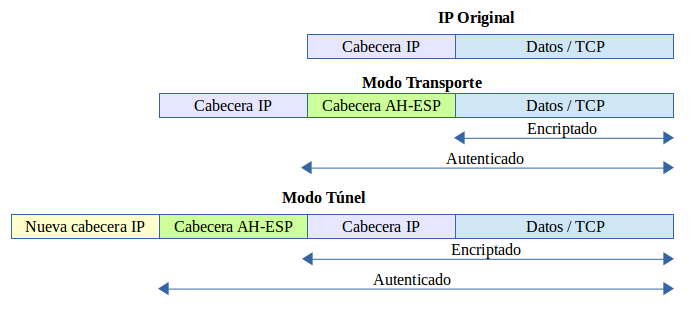
\includegraphics[width=5.00in]{images/IPsec.png}}
		}
		\caption{Ejemplo de paquetes IP con diferentes niveles de seguridad de encapsulación}
		\label{fig:norm_Daugman}
	\end{figure}

El protocolo de túnel hace de las VPNs una gran opción si el objetivo es la protección de nuestra información personal. 
Permite a un usuario conectarse a Internet con una dirección IP que no es parte de la red local. La \textbf{tunelización} funciona encriptando y encapsulando los datos, es decir, lo que proporciona un tercer y muy buscado beneficio: \textbf{el anonimato y la privacidad}. 

La forma en la que opera es un poco más compleja que con el modo de transporte, los paquetes que contienen la información que realiza el cifrado y el servicio de entrega se llevan a cabo dentro de la carga útil del mensaje original, pero operan a un nivel más alto que la propia carga útil, creando un escudo formado desde dentro y seguro de las influencias externas. Los mejores servicios cifrarán todo el paquete, el marcador de identificación y todo; a continuación, volverán a encapsularlo con una nueva dirección IP y marca de identificación para obtener una completa privacidad.

El modo túnel recoge su nombre de la forma en la que una red VPN opera:

  		\begin{figure}[h]
  			\centerline{
  				\mbox{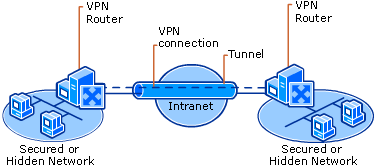
\includegraphics[width=3.50in]{images/vpn.png}}
  			}
  			\caption{Fuente: \textit{https://technet.microsoft.com/pt-pt/library/cc779919(v=ws.10).aspx}}
  			\label{fig:norm_Daugman}
  		\end{figure}
 
 Hoy en día, se usan diferentes tecnologías VPN, cada una con sus pros y sus contras.
 
 Entre todas ellas las más destacables son:
 
 \begin{itemize}
 	\item PPTP: \textit{Point to Point Tunneling Protocol}, la cual está bajo licencia de Microsoft(fue el primer protocolo de VPN compatible con Windows), crea una red privada virtual en redes dial-up. 
 	
 	Su implementación requiere poca sobrecarga de cómputos, lo cual lo hace uno de los protocolos de VPN \textbf{más rápidos} disponibles actualmente.
 	El problema con esta tecnología reside en que \textbf{no es del todo segura}. Aunque ahora normalmente utiliza una encriptación de 128 bits, existen varias vulnerabilidades de seguridad, con la posibilidad de una autenticación MS-CHAP v2 no encapsulada como la más grave. Con todo esto, una red que usase PPTP podría ser decodificada en apenas días.
 	La misma Microsoft, pese a haber corregido el fallo de seguridad, no recomienda el uso de este protocolo, y recomienda el uso de SSTP o L2TP.
 	
 	\item L2TP y L2TP/IPsec: El protocolo de túnel de capa dos, normalmente se implementa con los protocolos IPsec (explicados anteriormente) para encriptar datos antes de la transmisión, a fin de proveer a los usuarios privacidad y seguridad. Todos los dispositivos y sistemas operativos modernos compatibles con VPN tienen L2TP/IPsec incorporado. La configuración es tan rápida y fácil como la de PPTP, sin embargo en ocasiones puede ser problemático en el caso de que usar un cortafuegos NAT restrictivo.
 	
 	\item L2TP y L2TP/IPsec: El protocolo de túnel de capa dos, normalmente se implementa con los protocolos IPsec (explicados anteriormente) para encriptar datos antes de la transmisión, a fin de proveer a los usuarios privacidad y seguridad. Todos los dispositivos y sistemas operativos modernos compatibles con VPN tienen L2TP/IPsec incorporado. La configuración es tan rápida y fácil como la de PPTP, sin embargo en ocasiones puede ser problemático en el caso de que usar un cortafuegos NAT restrictivo.
 	Por el momento, \textbf{no hay vulnerabilidades importantes }relacionadas con la encriptación por IPsec, pero John Gilmore,  miembro fundador y especialista en seguridad de la Electric Frontier foundation, afirma que es probable que el protocolo sea debilitado intencionalmente por la NSA.
 	
 	\item SSTP: Secure Socket Tunneling Protocol fue presentado por Microsoft en el Service Pack 1 de Windows Vista. Este estándar está además ahora disponible para SEIL, Linux y RouterOS, aunque sigue siendo principalmente una plataforma únicamente para Windows. 
 	Utiliza SSL v3, y no tendría por qué tener problemas de seguridad aparentes. Sin embargo, hay que recordar que es propiedad de una gigante como Microsoft, y no puede ser analizado en busca de ingresos clandestinos.
 	
 	\item IKEv2: Internet Key Exchange, en su segunda versión, es un protocolo de túnel basado en IPsec, fue desarrollado por Cisco y Microsoft.
 	Los dispositivos móviles son los más beneficiados con IKEv2 ya que el protocolo de movilidad y multioproveedor que se ofrece en forma predeterminada lo hace extremadamente flexible para cambiar de redes. Pese a que IKEv2 está disponible en menos plataformas comparado con IPsec, tiene buena reputación en términos de estabilidad, seguridad y rendimiento.
 	
 	\item OpenVPN: Es un estándar \textit{open-source }relativamente nueva, utiliza los protocolos SSLv3/ TLSv1 y biblioteca OpenSSL para brindar a los usuarios una solución de VPN confiable y potente. El protocolo tiene amplia capacidad de configuración, lo que hace que sea muy difícil de bloquear para servicios como Google.	La principal ventaja de esta tecnología es que OpenSSL, la biblioteca que utiliza, soporta\textbf{ múltiples algoritmos criptográficos }tales como 3DES, AES, Camellia, Blowfish, CAST-128 y más, aunque Blowfish o AES son utilizados casi exclusivamente por proveedores de VPN.
 	La rapidez con la que se desempeña el protocolo OpenVPN depende del nivel de encriptación utilizado, pero normalmente es más rápido que IPsec. Por contra, la configuración, es complicada en comparación con L2TP/IPsec y PPTP.
 \end{itemize}
 
 \subsubsection{OpenVPN}
 
	Una vez explicadas las diferencias de este estándar con algunas de sus alternativas, vamos a ver cómo funciona éste en una plataforma GNU/Linux.
	
	Lo primero que conviene hacer es cambiar \textbf{el servidor DNS por defecto.}
	Esto, pese a que no es algo explícito ni directamente relacionado con el funcionamiento de la VPN, sí es recomendado. En determinadas ocasiones, pese a utilizar un servicio VPN, la traducción de nombre de dominios a su correspondiente IP numérica (dicha petición debería hacerse mediante el túnel VPN) puede hacerse erróneamente por medio del proveedor de Internet. Ésto se conoce como \textbf{DNS leak}. 
	Para evitarlo hay muchas soluciones. Entre ellas, algunos clientes de VPN (como Mullvad) permiten activar un campo en la configuración que evita estos problemas. Otra forma, en sistemas Unix, es acceder al archivo de configuración localizado en /etc/dhcp/dhclient.conf, descomentar la línea:
	
	{\fontfamily{bch}\selectfont 
		\#prepend domain-name-servers 127.0.0.1;
	}

	Evidentemente, hay que cambiar la dirección del servidor de DNS que utilizaremos. Podemos encontrar múltiples servidores, todos ellos seguros, en \textit{https://www.opendns.com}.
	
	Tras esto (y reiniciar la red, evidentemente) podemos utilizar openVPN sin riesgo a que ocurran DNS-leaks.
	
	Utilizar openVPN es tan sencillo como llamar al programa por línea de comandos pasándole como argumento un fichero \textit{.ovpn}, los cuales podemos conseguir, por ejemplo, en \textit{openvpn.com}.
	
	Una duda que puede surgirnos es, si nuestro objetivo es mejorar nuestra privacidad y anonimato ¿cuál es una mejor alternativa, una VPN ó el uso de un proxy? 
	
	Lo cierto es que, como veremos, no son las únicas opciones a la hora de obtener un mayor grado de anonimización.Sin embargo, la respuesta no es rotunda puesto que depende de qué servicio VPN y qué proxy se utilice.
	
	El uso de un proxy, hay tres protocolos principales, que como hemos visto son HTTP/HTTPS y SOCKS,
	Si usamos un proxy HTTP ó SOCKS, el uso de éste no proveerá de ningún tipo de encriptación de los datos, mientras que los proxies HTTPS ofrecen un nivel de encriptación igual que una web que funcione con el protocolo SSL. Además, por lo general, el uso de los proxies (sobre todo si se usan cadenas de los mismos) implican una muy baja velocidad de conexión.
	
	El caso de los VPN, hasta el momento es imposible interceptar el tráfico que circula por su túnel. Sin embargo, ésto produce un \textbf{único punto de fallo}, y es el servicio VPN. Es necesario asegurarse de que el servicio VPN que utilizamos no guarda logs ni otros datos, pues en el momento en el que dichos logs saliesen a la luz, estaríamos totalmente expuestos.
	
\subsection {Tor}
	
El uso de Tor supone una tercera entre muchas alternativas para mejorar nuestra privacidad y anonimato.

Tor es un software libre que permite defenderte contra el análisis de tráfico, y avoca por la privacidad y libertad del usuario. La forma en la que lo consigue es haciendo "rebotar" nuestra información en distintos \textbf{nodos Tor} intermedios con el objetivo de que el origen de la información se oculte lo máximo posible.
\lsection{Herramientas de identificación de usuarios} \label{sec:identificacion}
\subsection{Introducción}
\lsection{Debate social}
\label{sec:social}
\subsection{LOPD GPDR proteccion de datos ley reciente}

\newpage \thispagestyle{empty} % Página vacía 